\documentclass[a4paper,10pt]{article}

\usepackage[T1]{fontenc}
%%\usepackage{charter}
\renewcommand{\ttdefault}{pcr}

\usepackage[pdftex]{graphicx}
\usepackage{listings}

\title{Prototype A1}
\author{Alkis Gotovos}

\begin{document}
\lstset{language=Erlang, basicstyle=\small \ttfamily}

\begin{titlepage}
\maketitle
\thispagestyle{empty}
\end{titlepage}

\section{Introduction}
The aim of this document is to describe the structure and features
of a fully functional prototype for the Erlang concurrency testing tool that we
intend to develop. Our rationale is to use this prototype (PRA1) to gain insight
into the inner workings of our main project and detect potential pitfalls
as early as possible.

In the following sections we present the subset of functionality that we
shall implement in PRA1, as well as an overview of its architecture
(which possibly forms a structural preview for our main project).

\section{Functionality}
Being the very first prototype, PRA1 shall only implement a core subset of the
overall functionality. Specifically, we shall consider the following Erlang
"constructs" for now:
\begin{itemize}
	\item The \lstinline+spawn/1+ BIF
	\item The send (\lstinline+!+) expression, i.e. \lstinline+Expr1 !    Expr2+
	\item The simple \lstinline+receive+ expression (not containing an \lstinline+after+ clause),
	i.e.
	\begin{lstlisting}
    receive
    Pattern1 [when GuardSeq1] ->
        Body1;
    ...;
    PatternN [when GuardSeqN] ->
        BodyN
    end
	\end{lstlisting}
\end{itemize}

The current implementation viewed as a black box, shall accept a single erlang module for analysis
and output a log text file, containing all possible schedules w.r.t. the aforementioned "constructs".

\section{Structure}

\begin{figure}[htb]
	\centering
	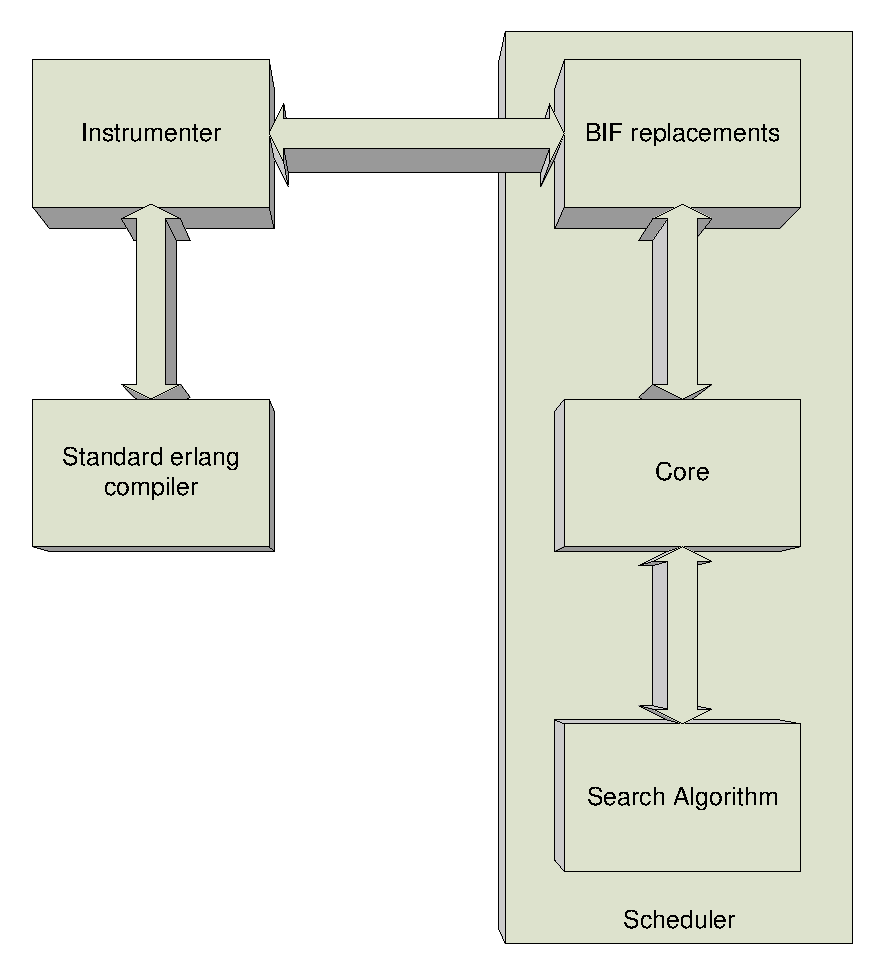
\includegraphics[width=300px]{PRA1}
	\caption{Module structure and interaction}
\end{figure}


\end{document}